 \chapter{Использование в диалоговой платформе {DeepPavlov Dream} многозадачных моделей}\label{ch:mtldream}
В данной главе решалась следующая \textbf{задача} -- \textbf{Интегрировать рассмотренные в диссертации многозадачные нейросетевые архитектуры в диалоговую платформу, оценить применимость данных архитектур и провести их сравнительный анализ на основании результатов на задачах данной платформы.}

Под диалоговой платформой в контексте выполнения данной задачи понималась диалоговая платформа DeepPavlov Dream. Эта платформа подробно описана в следующем разделе.

\section{Диалоговая платформа DeepPavlov Dream}\label{ch:dream}
Необходимость использования многозадачных нейросетевых моделей для обработки естественного языка обуславливает необходимость экономии вычислительных ресурсов при обрабоаатке естественного языка. Одной из ключевых областей, в которой широко применяются новейшие модели для обработки естественного языка, являются диалоговые системы.  Использование нейросетевых моделей, включая многозадачные, в диалоговых системах изучалось автором данном диссертационной работы на примере задач диалоговой платформы DeepPavlov Dream. Данная платформа является результатом развития диалоговой системы DREAM, вышедшей в полуфинал конкурсов «Alexa Prize Socialbot Grand Challenge 3» и «Alexa Prize Socialbot Grand Challenge 4»: после завершения этих конкурсов диалоговая система получила название DeepPavlov Dream и была выложена в открытый доступ, после чего продолжила свою эволюцию. Так как исходный код DeepPavlov Dream находится в открытом доступе, данный программный продукт является полноценной диалоговой платформой и может быть полезным для широкого круга разработчиков и исследователей.


Автор диссертационной работы принимал активное участие в работе над диалоговой платформой DeepPavlov Dream и системой DREAM. Так, автор оба раза был членом команды «DREAM» в конкурсе Alexa Socialbot Grand Challenge, что описано также в работах~\cite{dream1,dream1_trudy,dream2}. В даннм разделе описано устройство диалоговой системы {DREAM} и её эволюция в течение двух конкурсов, при этом акцент по возможности сделан на ее компоненты, являющиеся личным вкладом автора. При этом личный вклад автора не исчерпывается работой только над упомянутыми в статье компонентами -- он включал в себя также анализ работы других навыков диалоговой платформы и помощь в их отладке.


\subsection{Конкурс Alexa Prize Socialbot Grand Challenge}

Компания Amazon проводила конкурс Alexa Prize Socialbot Grand Challenge с 2017 года. Alexa Prize Socialbot Grand Challenge -- это конкурс диалоговых систем широкого профиля, разрабатываемых университетскими командами из разных стран. Предназначение данных систем -- общение с пользователями голосовых колонок Alexa от Amazon на различные популярные темы. Режим разговора с диалоговой системой во время конкурса включался командой «Alexa, let’s chat».

После окончания разговора пользователю предлагалось оценить качество диалога по шкале от 1 до 5 ( 1 -- наименьшая оценка, 5 -- наибольшая). 

Финальной целью данного конкурса являлось достижение следующих показателей: среднее качество диалога больше 4, среднее время разговора больше 20 минут. В связи со сложностью достижения этой цели, конкурс был сделан поэтапным. Каждый год компания Amazon организовывала Alexa Prize Challenge, в котором из большого числа заявок (несколько сотен в год) отбиралось до 10 университетских команд для участия в конкурсе. 

Данный конкурс имел продолжительность более полугода и состоял из следующих этапов:
\begin{itemize}
\item Подготовительный период. Команды работают над своими диалоговыми системами и тестируют их внутри своих команд.
\item Период бета-тестирования на пользователях-сотрудниках Amazon.
\item Период начальной обратной связи (англ: Initial Feedback Period). В этот период системы-участники впервые становятся доступными обычным пользователям колонок, которые могут общаться с этими системами и ставить им ту или иную оценку. Рейтинги в этот период еще не влияют на отбор команд для прохода в следующий этап.
\item Период четвертьфинала(англ: Quaterfinals). По рейтингам за последнюю неделю четвертьфиналов отбираются команды для прохода в полуфиналы.
\item Период полуфинала(англ: Semifinals). По среднему рейтингу за все время полуфиналов отбираются команды для прохода в финалы.
\item Период финала(англ: Finals). Во время финалов специально обученное жюри проводит слепое тестирование диалоговых систем. По результатам данного тестирования жюри выбирает итогового победителя. При этом изменения кода в периоде финалов уже запрещены.
\end{itemize}

Команда Московского физико-технического института «DREAM» была отобрана для участия в конкурсах «Alexa Prize Challenge 3»~\cite{na_website_ndh} и «Alexa Prize Challenge 4»~\cite{na_website_ndi}. В каждом из этих конкурсов автор данной диссертационной работы принимал активное участие в этой команде. Диалоговая система {DREAM} подробнее описана в~\cite{dream1, dream1_trudy, dream2}.

\begin{figure}[ht]
  \centerfloat{
    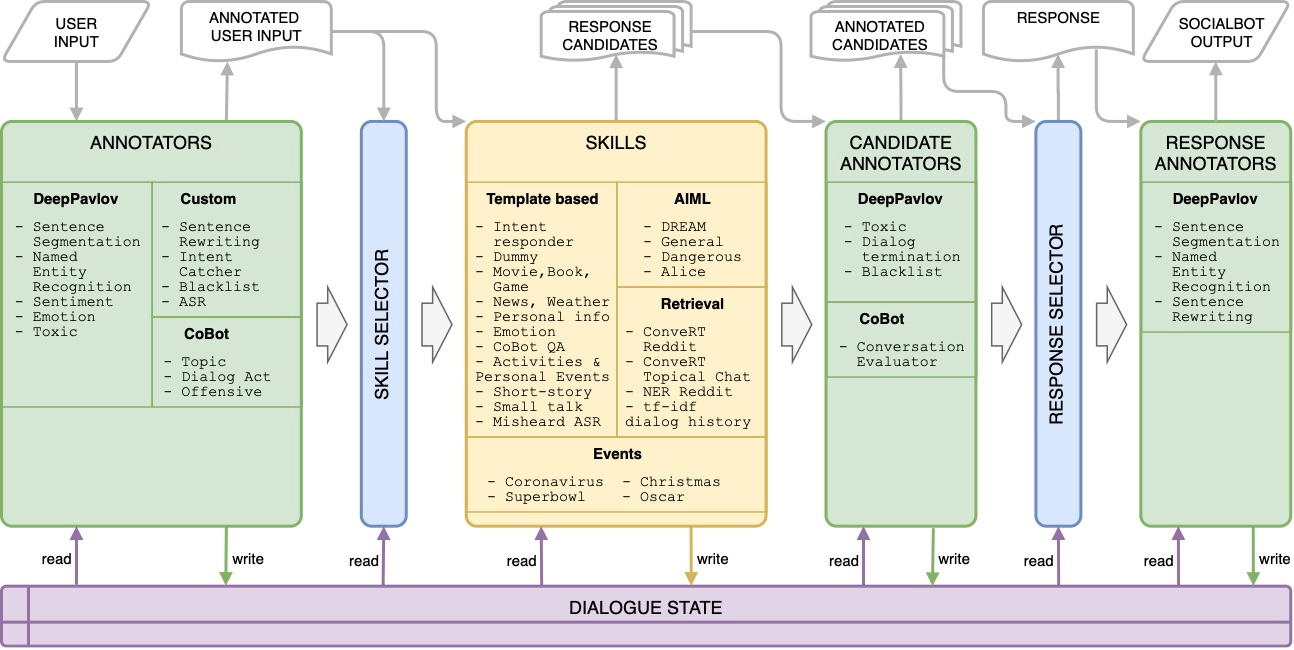
\includegraphics[width=\textwidth]{images/Alexa1_.png}
  }
  \caption{Архитектура диалоговой системы {DREAM} в конкурсе «Alexa Prize Challenge 3»}\label{fig:Alexa1}
\end{figure}


Диалоговая система {DREAM} для участия в конкурсе Alexa Prize Challenge 3 разрабатывалась с нуля, на основе фреймворка DeepPavlov Agent --  разработки сотрудников лаборатории нейронных систем и глубокого обучения МФТИ. Разработка {DREAM} велась с 2019 года.

В связи с тем, что DeepPavlov Agent на тот момент находился на раннем этапе своего развития, код DeepPavlov Agent был скопирован непосредственно в репозиторий диалоговой системы и редактировался непосредственно в этом репозитории.

Задача развертывания диалоговой системы на большое число пользователей решалась с использованием Docker Compose~\cite{na_website_ndk}.

На Рисунке~\ref{fig:Alexa1} представлена верхнеуровневая архитектура диалоговой системы {{DREAM}} на момент завершения ее участия в конкурсе «Alexa Prize Challenge 3». Реплика, поступающая модели {{DREAM}} на вход, вместе с состоянием диалога, в котором хранится информация о диалоге вместе со всеми аннотациями (Dialog State) проходит через аннотаторы (Annotators). На основе аннотаций, полученных от аннотаторов, модуль Выборщик навыка (Skill Selector), пользуясь оригинальным алгоритмом, выбирает навыки (Skills) для генерации кандидатов на возможный ответ бота. Каждый навык генерирует возможный ответ с определенной степенью уверенности. Данные ответы фильтруются при помощи аннотаторов кандидатов на ответ, этим ответам присваиваются очки от модуля Оценка разговора Cobot (Cobot Conversation Evaluator). На основе аннотаций, очков и фильтрации оригинальный разработанный модуль Выборщик ответа (Response Selector) выбирает финальный ответ-кандидат. Данный ответ бота проходит через постаннотаторы (Postannotators) и в таком виде уже доводится до пользователя.

Диалоговая система принимает реплики пользователя на вход в виде текстовой транскрипции. При этом модуль тестовой транскрипции предоставляется компанией Amazon «из коробки». Заметим, что ошибки этого модуля сами являлись причиной определенного процента ошибок диалоговой системы {DREAM} (около 10 процентов).

На вход модели, после каждой реплики пользователя, поступает список слов, которые распознала модель. Каждому слову соответствует степень уверенности распознавания речи. Например, после фразы пользователя «alexa how old are you» модель получает на вход от модуля текстовой транскрипции список следующего вида: [(«alexa» : 0.95),«how» :0.96, («old» :0.8), («you» : 0.9)]. Заметим, что подобные списки не разделены по предложениям и не имеют пунктуацию. Поэтому, чтобы реплики обрабатывались лучше, диалоговая система использует аннотатор сегментации предложений (Sentence Segmentation) для восстановления пунктуации и разделения реплик на предложения. Кроме этого диалоговая система использует также модель для переписывания предложений (Sentence Rewriting), заменяющую местоимения на сущности, которые были упомянуты ранее в диалоге.


\subsubsection{Первый этап разработки: навыки и аннотаторы}

На первом этапе разработки ключевыми интегрированными в бота {{DREAM}} навыками и аннотаторами, помимо упомянутых выше, являлись:

Удаленные сервисы, предоставленные командой «Amazon» --  классификатор Cobot Topics, классификатор диалоговых актов и тем Cobot DialogAct, Вопросы и ответы Cobot (Cobot QA)

Имеющиеся в открытом доступе навыки для диалога на общие темы, построенные на правилах -- Alice, AIML Chit-Chat(встроенный под названием program-y). В дальнейшем данные навыки многократно совершенствовались -- как в связи с паттернами ответов пользователей, наблюдавшихся в реальных диалогах с системой {DREAM}, так и в связи со специфичными требованиями правил~\cite{na_website_ndg}. Помимо этого, был добавлен навык Ответ на интенты (Intent Responder) для ответа на конкретные интенты и навыки-«затычки» Навык-Затычка (Dummy Skill) и Диалоговый навык-затычка (Dummy Skill Dialog).

\subsubsection{Аннотаторы}

На следующих этапах разработки добавлялись иные аннотаторы реплик пользователя, часть из которых ( см. Рисунок 10) также использовалась как постаннотаторы для аннотации реплик диалоговой системы. Такие аннотаторы включают в себя:
\begin{itemize}
\item Детектор запрещенных слов (Blacklisted Words Detector) -- используется для обнаружения нецензурных или просто оскорбительных слов или выражений. Данный аннотатор основан на регулярных выражениях и использует заданный вручную список слов.

\item Классификация интентов (Intent Catcher) -- используется для обнаружения одного из 22 интентов. Данный аннотатор работает как на наборе регулярных выражений, обновлявшемся вручную в течение конкурса, так и на модели Universal Sentence Encoder~\cite{cer_2018}.

\item Классификация токсичности (Toxic Classification) -- нейросетевой многометочный классификатор, определяющий, относится ли реплика к любому из следующих классов -- ненависть(identity\_hate), оскорбление(insult), обсценная лексика(obscene), очень токсичный(very\_toxic), секс(sexual\_explicit), угроза(threat), токсичный(toxic). Данный аннотатор основывается на модели «разговорный BERT»\cite{dp_conv_bert}, которая является частью библиотеки DeepPavlov и которая была дообучена на данных с Kaggle-соревнования «Jigsaw Unintended Bias in Toxicity Classification»~\cite{toxic_kaggle}.

\item Классификация тональности (Sentiment Classification) -- нейросетевой классификатор тональности, основанный на модели «разговорный BERT»~\cite{na_website_ndn}, обученной на наборе данных Stanford Sentiment Treebank~\cite{sst}. Классификатор распознает три класса -- положительный, отрицательный, нейтральный.

\item Классификация остановки диалога (Dialog Termination) -- нейросетевой классификатор -- предсказатель завершения диалога. Ближе к концу конкурса, когда у команды {{DREAM}} накопилась достаточно большая база диалогов(сотни тысяч), на основе вышеупомянутой модели «разговорный BERT» была обучена модель-постаннотатор, которая для каждой реплики бота определяла вероятность завершения пользователем диалога после этой реплики. На основании очков от этой модели Выборщик ответа фильтровал реплики-кандидаты. Данная модель является личным вкладом автора диссертационной работы.
%todo gossip skill слухи grounding skill обоснование диалога

\item Классификация эмоций (Emotion Classification) --  нейросетевой классификатор эмоций, основанный на модели «BERT-Base-uncased», обученный на наборе данных с Kaggle страницы Eray Yildiz~\cite{na_website_ndp_emo}. Эти данные содержали 6 классов -- ярость, грусть, любовь, радость,удивление, любовь. Для корректной работы классификатора необходимо, чтобы в данных присутствовали также примеры, принадлежащие нейтральному классу. Для этого были добавлены примеры из набора данных ScenarioSA~\cite{scenariosa}, которым был присвоен нейтральный класс. Итоговый набор данных сохранен по адресу~\cite{na_website_ndo_emo}.
\end{itemize}
Модель для классификации эмоций является личным вкладом автора, в связи с чем она описывается более подробно, чем остальные. После первой эпохи при обучении с оптимизатором Adam и скоростью обучения 5*10-5 данной моделью была достигнута точность 94.2\% на валидационном наборе данных. Классификатор обучался как многометочный, но для метрик предсказанным считался самый вероятный класс. Матрица ошибок данного классификатора представлена ниже.


\begin{table}[htbp]
\centering
\caption {Матрица ошибок классификатора эмоций из Alexa Prize Challenge 3}
\label{tab:dream1}% label всегда желательно идти после caption
\resizebox{\textwidth}{!}{%
\begin{tabular}{|c||c|c|c|c|c|c|c|}
\hline
\multirow{2}{*}{Настоящий класс} & \multicolumn{7}{c|}{Предсказанный класс} \\
\cline{2-8}
  & Ярость & Страх & Удовольствие & Любовь & Грусть & Удивление & Нейтральный\\
\hline
\hline
Ярость & 5933 & 49 & 38 & 2 & 22 & 291 & 1 \\
\hline
Страх & 263 & 4624 & 18 & 0 & 12 & 1 & 419 \\
\hline
Удовольствие & 17 & 5 & 14697 & 1138 & 4 & 27 & 112 \\
\hline
Любовь & 1 & 1 & 14 & 3867 & 0 & 4 & 1 \\
\hline
Грусть & 6 & 3 & 2 & 1 & 3109 & 0 & 0 \\
\hline
Удивление & 48 & 229 & 36 & 7 & 9 & 13725 & 16 \\
\hline
Нейтральный & 1 & 2 & 44 & 0 & 0 & 2 & 1609 \\
\hline
\end{tabular}
}
\end{table}



Результат данного классификатора в данном конкурсе использовался навыками обсуждения эмоций и обсуждения коронавируса, которые будут подробнее описаны в разделе~\ref{dream:1:closed}.

\subsubsection{Навыки открытого домена}

В течение конкурса командой {{DREAM}} активно создавались навыки открытого домена для того, чтобы как можно большее число тем было покрыто хотя бы на минимальном уровне. Были созданы следующие навыки открытого домена:

Ранжирующий навык TF-IDF (TF-IDF Retrieval) использует диалоги за прошлый месяц, получившие хорошую оценку (5) и плохую (1-2). Получая на вход пользовательскую фразу, он строит TF-IDF векторное представление~\cite{tfidf} данной фразы и выбирает фразу бота из получивших хорошую оценку диалогов, максимально близкую по косинусному расстоянию к данной пользовательской фразе и не принадлежащую при этом к множеству диалогов, получивших плохую оценку. Уверенность данного навыка соответствует косинусному расстоянию между векторными представлениями фразы пользователя и бота, но не превышает при этом некоторе постоянное значение. Векторизатор для получения представлений был обучен на конкатенации наборов данных TopicalChat\cite{topicalchat}, PersonaChat~\cite{personachat} и Wizard of Wikipedia~\cite{wow}. Разработка данного навыка относится к личному вкладу автора.  Это единственный навык, который интегрировал в себя новые диалоговые данные из конкурса в автоматическом режиме.

В дальнейшем было также обучено подмножество аналогичных навыков, покрывающих разные темы из набора данных TopicalChat  -- книги, развлечения, мода, фильмы, музыка, политика, технологии, спорт и животные -- каждый на основе соответствующего набора данных из TopicalChat.

Генеративный навык является другой разработкой автора. В данном навыке использовалась модель типа GPT\cite{radford_2018_gpt} с добавлением «персоны» для улучшения качества генерации модели. Данная модель дообучалась в различных экспериментах на PersonaChat, на TopicalChat, на Wizards of Wikipedia или на сочетании всех этих трех наборов данных . В качестве персоны(сообщения, исходя из которого генерировалась дальнейшая реплика) в данных экспериментах использовались в качестве условия для генерации, соответственно, персона для примеров из набора данных PersonaChat, одно из предложений, на которое была отсылка в Wizards of Wikipedia(далее -- WOW) для примеров из Wizards of Wikipedia и один из наиболее релевантных фактов, связанных с этой фразой(по TF-IDF) для примеров из TopicalChat. Максимальная длина предложения со всей диалоговой историей и персоной равнялась 512 токенов.  Данная модель продолжает проводившуюся ранее автором работу над диалоговой моделью«с персоной»~\cite{Болотин_Карпов_Рашков_Шкурак_2019}.

Несмотря на хорошую перплексию (см. Таблицу~\ref{tab:dream2}), навык не был включен в систему {{DREAM}} из-за своей недостаточной логической консистентности.

\begin{table}[htbp]
\centering
\caption {Точность (перплексия) для генеративного навыка.}
\label{tab:dream2}% label всегда желательно идти после caption
\resizebox{\textwidth}{!}{%
\begin{tabular}{|c||c|c|c|c|}
\hline
\multirow{2}{*}{Обучающие данные} & \multicolumn{4}{c|}{Метрики} \\
\cline{2-5}
 & PersonaChat & TopicalChat & WOW & 3 набора данных \\
\hline \hline
PersonaChat & 90(12.3) & - & - & - \\
\hline
TopicalChat & - & 96(9.7) & - & - \\
\hline
WOW & - & - & 86.7(27.2) & - \\
\hline
3 набора данных & 86(14.2) & 92(11.6) & 83(31.5) & 92(16.3) \\
\hline
\end{tabular}
}
\end{table}



ConveRT Reddit -- нейросетевой ранжирующий навык, обученный на наборе комментариев с сайта REDDIT~\cite{na_website_ndu} (отфильтрованном аннотаторами Оценка разговора Cobot и Классификация токсичности 80 тыс.примеров) и использующий нейросетевую модель CONVERT~\cite{henderson_2019} для получения векторных представления реплики и контекста(конкатенации предыдущих реплик). Данная модель вместо модели BERT была выбрана в целях экономии вычислительных ресурсов и для повышения быстродействия.

\subsubsection{Навыки закрытого домена}\label{dream:1:closed}

Тем не менее, вышеупомянутых навыков все еще в большинстве случаев было недостаточно для того, чтобы вести долгий, логически завершенный диалог на популярные темы. В связи с этим также был создан ряд навыков закрытого домена, основанных на правилах, использовании нейросетевых аннотаций и при необходимости делающий внешние запросы. Ниже описаны три навыка закрытого домена, являющиеся личным вкладом автора. Остальные такие навыки подробнее описаны в~\cite{dream1,dream1_trudy}

Навык обсуждения эмоций (Emotion Skill) возвращает шаблонные ответы на эмоции, обнаруженные аннотатором для классификации эмоций. В частности, навык может подсказать совет,рассказать шутку или успокоить пользователя. Основная часть навыка была разработана автором самостоятельно.

В начале февраля 2020 года года, несмотря на общее падение рейтингов диалоговой системы(вероятно, связанное  с беспокойством пользователей по поводу новой коронавирусной инфекции), улучшение навыка обсуждения эмоций помогло повысить медианное время диалога с 58 до 73 секунд.

Навык обсуждения книг (Book Skill), используя базу данных Amazon Evi~\cite{na_website_nds}, находит названия книг и фамилии авторов. Используя данные именованные сущности, навык поддерживает разговор о данных книгах либо авторах. Помимо этого, навык также может рекомендовать книги, используя информацию из базы данных GoodReads~\cite{na_website_ndt} и аннотации из модели Cobot. Одной из технических проблем при разработке данного навыка являлось то, что некоторые названия книг заставляли реагировать и навык классификации книг, и навык классификации эмоций. Проблема была решена при помощи изменения уверенности навыка классификации книг в таких ситуациях.

В работе~\cite{dream1} показано, что использование Навыка для обсуждения книг и описанного выше Ранжирующего навыка TF-IDF помогло повысить рейтинг диалоговой системы в декабре 2019 года с 3.01 до 3.19.  В конце января-начале февраля 2020 года добавление истории диалога в Ранжирующий навык TF-IDF помогло дополнительно повысить рейтинг диалоговой системы до 3.25.

Навык обсуждения коронавируса (Coronavirus Skill) был добавлен на завершающем этапе конкурса, когда в связи с эпидемией COVID-19 (дело происходило в марте-июне 2020 года) пользователи стали часто поднимать эту тему в разговорах с диалоговой системой {DREAM}. Навык использовал данные о случаях коронавируса и смертях от него, взятых из Центра системной научной инженерии Университета Джона Хопкинса~\cite{na_website_ndr}. Навык использует факты, сравнения и научно обоснованные советы для того, чтобы успокоить пользователя с учетом его возраста. Навык использует аннотации от модели для классификации эмоций.

 Прирост рейтинга диалоговой системы в начале марта 2020 года был, вероятно, связан с добавлением и улучшением навыка обсуждения коронавируса.

Технические решения, аналогичные применявшимся автором работы в различных сценарных навыках (анализ паттернов в тексте, основанный на правилах), были применены также в сервисе для сканирования текстов texter-ocr-cv-nlp-microservice, на который был получен патент~\cite{Дуплякин_Дмитрий_Ондар_Ушаков_2021}.

\subsubsection{Выборщик ответа и Выборщик навыков}

При большом числе сценарных навыков, у многих пользователей тем не менее в середине конкурса возникали трудности с тем, чтобы «попасть» в какой-то конкретный навык. В связи с этим диалог часто становился логически неконсистентным. Для решения данной проблемы был реализован метод«направляющих вопросов», подразумевающих в качестве ответа мнение пользователя о заданной теме и/или выбор пользователем конкретной темы для обсуждения (фильма, книги, игры). Данные вопросы могли добавляться как на уровне навыка, так и на уровне Выборщика ответа. Как показано в~\cite{dream1}, использование подобного метода помогло повысить рейтинг диалоговой системы.
Выборщик навыков основан на постоянном включении нетематических навыков, включении тематических навыков при определенных условиях на аннотации реплики пользователя и использовании специального режима при обработке реплик, классифицированных классификатором токсичности как токсичные или просто принадлежащим к «острым» темам. Подробнее данный алгоритм описан в работе~\cite{dilya_thesis}.
Выборщик ответа в начале участия команды {{DREAM}} в конкурсе просто выбирал навык с максимальной уверенностью. В дальнейшем туда были интегрированы оценки от Оценки разговора Cobot, фильтрация с использованием постаннотаторов и набор иных эвристик. Подробнее данный алгоритм описан в той же работе~\cite{dilya_thesis}.

\subsection{Архитектура диалоговой системы {{DREAM}} в  «Alexa Prize Challenge 4»}


\begin{figure}[ht]
  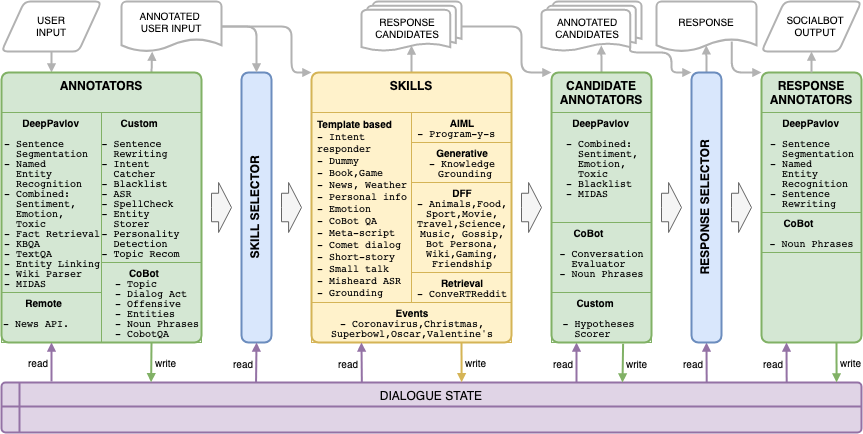
\includegraphics[width=\textwidth]{images/Alexa2_.png}
  \caption{Архитектура диалоговой системы {{DREAM}} в конкурсе«Alexa Prize Challenge 4»}\label{fig:Alexa2}
\end{figure}
Диалоговая система {{DREAM}} для участия в конкурсе следующего, 2021 года основывалась на доработанной системе прошлого года. Её схема представлена на рисунке~\ref{fig:Alexa2}.


Задача развертывания диалоговой системы решалась с использованием Kubernetes~\cite{kubernetes}.
Ключевые принципы работы диалоговой системы остались прежними, однако ее аннотаторы и навыки поменялись следующим образом.

\subsubsection{Изменения, связанные с аннотаторами}\label{dream:2:ann}

Одним из главных изменений, сделанных в диалоговой системе {DREAM}, являлась оптимизация вычислительных мощностей для экономии видеопамяти. Это было связано с высокими издержками на эксплуатацию данных мощностей -- каждый месяц расходовалось «кредитов» вычислительных мощностей на сумму до 9 тысяч долларов США. Для данной оптимизации шесть моделей-классификаторов:классификаторы эмоций, тональности, токсичности, а также классификаторы тем Cobot (Cobot Topics) и диалоговых актов Cobot (Cobot DialogAct)\footnote{Этот классификатор считался за 2, т.к возвращал тему и интент.} были объединены в один классификатор Combined Classifier. В условиях острого дефицита временных ресурсов, связанного с быстрой динамикой конкурса, был выбран способ реализации многозадачного обучения «Независимые метки» из статьи ~\cite{pseudolabel}, описанный также в главе~\ref{ch:pseudolabel}. Подробнее эксперименты, связанные с обучением данной модели, описаны ниже в главе~\ref{ch:mtldream}. Данная модель использовалась как постаннотатор всё время конкурса, а как классификатор пользовательских фраз -- при условии, что получение аннотаций от CoBot невозможно или задерживается (т.к модель CoBot имеет лимит на количество входящих запросов, такие ситуации возникали),  Данная модель является личным вкладом автора диссертационной работы.

Так как использование многозадачных моделей в диалоговой системе {DREAM} было продиктовано задачами этой платформы, задачи платформы {DREAM} пригодны для изучения прикладного применения многозадачных нейросетевых моделей.

Другим важным изменением является добавление классификатора диалоговых актов MIDAS (MIDAS Classifier), обученной на базе набора данных MIDAS~\cite{midas}. На первом этапе, в феврале, была интегрирована предоставленная авторами модель, на втором, в апреле, она была заменена собственной моделью, обученной только на семантических классах из данного набора данных, так как в {{DREAM}} используется только этот набор классов.


Полный список используемых семантических классов:
\begin{itemize}
\item открытый вопрос/мнение (open\_question\_opinion)
\item открытый личный вопрос(open\_question\_personal)
\item вопрос да/нет(yes\_no\_question)
\item вопрос для пояснения(clarifying\_question)
\item команда(command)
\item неверная команда (dev\_command)
\item признательность(appreciation)
\item мнение(opinion)
\item жалоба(complaint)
\item комментарий(comment)
\item утверждение(statement)
\item другие ответы(other\_answers)
\item положительный ответ(pos\_answer)
\item отрицательный ответ(neg\_answer)
\item открытый фактический вопрос(open\_question\_factual)
\end{itemize}
Обе модели были обучены на основе вышеупомянутой модели «разговорный BERT».  Работа над данным аннотатором тоже является личным вкладом автора диссертационной работы.

В конце февраля-начале марта 2021 года, как показано  в работе~\cite{dream2}, интеграция классификатора диалоговых актов MIDAS и изменение модели диалога в сторону более частого показа навыка обсуждения книг помогли поднять рейтинг диалоговой системы {{DREAM}} с $\sim$3.11 до $\sim$3.28.



Помимо этого, с середины конкурса использовался аннотатор Сущности Cobot (Cobot Entities) от Amazon как удаленный сервис. Данный аннотатор извлекал сущности и классифицировал их на несколько видов.
Также для рекомендации пользователю следующей темы (поддерживаемой имеющимся сценарным навыком) на основании текущего контекста был создан аннотатор Рекомендация тем (Topic Recommendation), подробно описанный в~\cite{dream2}.
Одним из ключевых изменений стала интеграция баз знаний -- добавление компонентов Связность сущностей(Entity Linking), Парсер Вики(Wiki Parser) и Ранжирование фактов(Fact Retrieval). Компонент Fact Retrieval получает для распознанных Cobot Entities сущностей факты из Википедии и WikiHow\cite{wikihow}.  Компонент Entity Linking соотносит каждую сущность, распознанную Cobot Entities, с идентификатором в системе WikiData~\cite{vrandei_2014}. Компонент Wiki Parser извлекает из этих идентификаторов триплеты -- наборы (субъект, соотношение, объект). Entity Linking и Wiki Parser широко использовались в навыках закрытого домена, таких, как навыки для обсуждения книг и сплетен, что позволило существенно улучшить их качество работы.
Также из всех навыков, которые делали запрос к удаленным сервисам(пример -- Вопросы и ответы Cobot, навык для обсуждения новостей News API Skill), модули запросов были оформлены как отдельные аннотаторы, что позволяло делиться полученной информацией между навыками.
Для того, чтобы определять, задал ли пользователь фактоидный вопрос (что в соответствии с алгоритмом, описанным в~\cite{dream2}, определяет приоритетность включения части упомянутых выше навыков), был также добавлен аннотатор классификации фактоидности. Этот аннотатор был основан на модели BERT, обученной на наборе данных YAHOO~\cite{yahoo_dataset}.
Помимо добавления новых навыков, инкрементальным улучшениям подвергались и старые навыки. В частности, автор работы большое время посвятил работе над Intent Catcher. 

\subsubsection{Изменения, связанные со сценарными навыками}
Одной из ключевых проблем, с которыми сталкивалась диалоговая система {{DREAM}} на момент проведения конкурса «Alexa Prize Challenge 3», являлось недостаточное количество сценарных навыков. (У команды-победителя сценарные навыки покрывали больше популярных тем на разговор хотя бы в несколько шагов, чем у команды {DREAM}). Те сценарные навыки, которые были реализованы, не были унифицированы распространялись на другие темы, в связи с чем качество разговоров бота на многие темы были низкими, также возникали сложности с отладкой навыка человеком, который его не разрабатывал. Для решения этой проблемы был разработан фреймворк для построения диалоговых систем Dialog Flow Framework(DFF)~\cite{dff}, позволяющий удобно записывать сценарий для диалогового графа. На основе данного фреймворка было разработано большое количество сценарных тематических навыков -- навыки для обсуждения животных (Animals Skill), еды (Food Skill), спорта (Sport Skill), науки (Science Skill), музыки (Music Skill), слухов (Gossip Skill), игр (Gaming Skill), личности бота (Bot Persona Skill), путешествий (Travel Skill), а также переведен на использование DFF навык для обсуждения фильмов (Movie Skill). Разработка подобных сценарных навыков позволила отключить использование соответствующих ранжирующих навыков, основанных на TF-IDF.

Личным вкладом автора диссертационной работы на данном этапе является существенное улучшение навыка для обсуждения книг (на основе запросов к Wikidata), навыка для обсуждения эмоций и аннотатора для классификации интентов (Intent Catcher).

Помимо навыков для обсуждения книг, эмоций и коронавируса,автор диссертационной работы отвечал еще за 2 сценарных навыка.
Одним из этих навыков был навык для обоснования диалога (Grounding Skill). Навык решал задачу установления взаимопонимания с пользователем. Используя информацию из истории диалога о том, какие сущности были упомянуты и какие были намерения у пользователя и у бота, навык генерирует шаблонную фразу-подтверждение. Этой фразой навык показывает, что бот понимает, о чем говорит пользователь. Например, если в аннотациях фразу есть сущность Fortnite и интент Opinion\_RequestIntent, навык выдает фразу «You wanted to hear my thoughts about Fortnite, am I correct?»

Другим навыком являлся навык для обсуждения слухов (Gossip Skill). В этом навыке отношение диалоговой к различным знаменитостям определялось случайно, и навык, используя WikiData и тональность реплики пользователя при его разговоре о той или иной знаменитости, обсуждал их. За работу над этим навыком автор диссертационной работы отвечал не все время (в отличие от первого навыка), но значительную часть времени.

\subsubsection{Изменения, связанные с навыками открытого домена}

Хотя сценарные навыки позволили вести логически связный разговор с пользователем значительное число диалогов и улучшить тем самым рейтинг этих диалогов, они все еще не могли покрыть все популярные темы и их подтемы. Для решения данной задачи были разработаны следующие навыки открытого домена, помимо упомянутых выше:
\begin{itemize}
\item Навык базы знаний (Knowledge Grounding Skill) -- нейросетевая генеративная модель ParlAI Blender 90M~\cite{roller_other_2020}, дообученная на наборе диалогов Topical Chat Enriched~\cite{hedayatnia_2020}.
\item Вики-навык (Wiki Skill) -- универсальный сценарный навык открытого домена. Он может обсуждать найденные в репликах пользователя сущности с использованием соответствующей страницы Википедии, что позволяет вести логически консистентный диалог по большому количеству популярных объектов, которые находятся за пределами внимания сценарных навыков.
\end{itemize}
\subsubsection{Изменения в Выборщике навыков и Выборщике ответа}

Ключевые изменения в Выборщике навыков и Выборщике ответа включали в себя более плавные переходы между парами тем; использование специфичных переходных фраз, относящихся к 2 темам одновременно, либо обычных связующих фраз как во время конкурса Alexa Prize Challenge 3, но вместе со связующими фактами.
Помимо этого, в связи с ростом количества и разнообразия сценарных навыков одной только уверенности перестало хватать для определения очередности их включения. В связи с этим сценарные навыки была добавлена приоритизация с возможными флагами продолжения вида «должен продолжать», «может продолжать» и «не может продолжать».
Подробнее обо всех изменениях в Выборщике навыков и Выборщике ответа можно прочитать в работе~\cite{dream2}.

\section{Использование многозадачных моделей в диалоговой системе {DREAM} и платформе {DeepPavlov Dream}}
В диалоговой платформе {DeepPavlov Dream} использовались разные типы многозадачных моделей - модель с одним линейным слоем, PAL-BERT и энкодер-агностичная модель. Использование моделей с одним линейным слоем началось ещё в диалоговой системе DREAM. В данном разделе описываются результаты этих моделей.
\subsection{Использование многозадачных моделей с одним линейным слоем }
\subsubsection{Использование многозадачных моделей с одним линейным слоем для объединения и замены классификаторов реплик}
Автором данной диссертационной работы многозадачные модели для задач диалоговой системы {DREAM} начали использоваться во время конкурса Alexa Prize Challenge 4. Необходимость использования многозадачных моделей была обусловлена как необходимостью экономии вычислительных ресурсов(в первую очередь видеопамяти), так и лимитом на количество ежедневных запросов к сервисам Amazon, который часто превышался в условиях интенсивных нагрузок конкурса.В связи с этим, была поставлена задача объединить шесть моделей -- модель для классификации эмоций, модель для классификации тональности, модель для классификации токсичности, модель для классификации тем Cobot (далее -- Cobot Topics), модель для классификации тем от аннотатора Cobot DialogAct (далее -Cobot DialogAct Topics) и модель для классификации интентов от аннотатора Cobot DialogAct (далее -- Cobot DialogAct Intents).

Первой версией многозадачной модели, использовавшейся для решения этих задач, являлась модель с одним линейным слоем, имеющая такую же архитектуру,
как и модель, описанная в главе~\ref{ch:pseudolabel}.

Заметим, что набор данных из конкурса Alexa Prize Challenge 3 для обучения модели имел следующую особенность -- все пользовательские фразы имели аннотации сразу от всех моделей. В связи с этим, модель BERT в первой серии экспериментов обучалась на этих данных, получая на вход предсказания этих моделей(сохранённые в архиве диалогов во время конкурса) в качестве меток. Иными словами, использовался подход, аналогичный подходу «Жесткие независимые метки» из главы~\ref{ch:pseudolabel}, но без объединения меток. 
 
Все имеющиеся данные были поделены в пропорции 90/8/2 между тренировочным, тестовым и валидационным наборами данных. Перед делением были отфильтрованы дубликаты среди фраз. В первом экспериментальном сеттинге каждой фразе присваивалась наиболее часто встречаемая метка для данной фразы и задачи (если встречалось более 1 метки).

В первой серии экспериментов сравнивались следующие способы обучения:
\begin{itemize}
\item Обучение отдельной модели BERT для каждой из задач
\item Обучение одной модели BERT для трех задач Cobot и другой -- для трех остальных задач
\item Обучение одной модели BERT для всех 6 задач
\end{itemize}

Все эти способы сравнивались не только друг с другом, но и (для не-Коботовских задач) с результатами оригинальной модели. 

Особо отмечаю, что «чистого» набора данных для решения Коботовских задач автор диссертационной работы не имел, а те диалоговые данные, что были доступны автору, было запрещено отдавать на разметку в связи с соображениями пользовательской приватности. По этой причине модели, заменяющие Коботовские сервисы (Cobot Topics, Cobot DialogAct Topics, Cobot DialogAct Intents) оценивались исключительно по соответствию своих предсказаний предсказаниям оригинальных моделей(на тестовой выборке). Соответственно, оригинальные модели Cobot Topics, Cobot Dialogact Topics и Cobot Dialogact Intents в рамках данного эксперимента(как и всех упомянутых ниже) имеют точность и взвешенный-F1, равные 1.

Модели для классификации эмоций, сентимента и токсичности оценивались на тестовых частях своих наборов данных\cite{sst},\cite{na_website_ndo_emo},\cite{toxic_kaggle} . 


Отметим также, что для каждой из задач могло быть предсказано больше 1 метки.
Максимальная длина предложения в проводимых экспериментах равнялась 32 токена, скорость обучения равнялась \num{1e-5}. Использовался оптимизатор AdamW с параметром decay, равным 0.01. В качестве F1-метрики использовался взвешенный-F1. Размер батча считался равным 128. Обучение модели проводилось без ограничений по числу эпох, но с остановкой в случае неулучшения средней точности в течение 5 эпох.
% « »
\begin{table}[htbp]
    \caption{Точность (взвешенный-F1) для многозадачной классификации для различных моделей. «1 в 1» означает оригинальные модели, «6 в 1» -- многозадачную модель с одним линейным слоем, обученную на аннотациях всех упомянутых в таблице классификаторов, «3 в 1 (Cobot)» -- многозадачную модель с одним линейным слоем, обученную только на аннотациях классификаторов Cobot Topics, Cobot DialogAct Topics и Cobot DialogAct Intents, «3 в 1 (не Cobot)» -- многозадачную модель с одним линейным слоем, обученную только на аннотациях остальных классификаторов(классификаторы эмоций, тональности и токсичности).}
    \label{mtldream:1}
    \centering
    \scalebox{0.95}{
    \begin{tabular}{|c|c|c|c|c|} 
    \hline
    \multirow{2}{*}{3адача} & \multicolumn{4}{c|}{Модели} \\
    \cline{2-5}
     & \textbf{1 в 1} & \textbf{6 в 1} & \textbf{3 в 1 (Cobot)} & \textbf{3 в 1 (не Cobot)}\\
    \hline
    Cobot Topics   & --- & 84~(83) & 82~(84) & --- \\
    \hline
    Cobot DialogAct Topics  & --- & 76~(64) & 78~(66) & --- \\
    \hline
    Cobot DialogAct Intents & --- & 69~(65) & 70~(67) & --- \\
    \hline
    Эмоции  & 92~(75) & 82~(60) & --- & 85~(67) \\
    \hline
    Тональность & 72~(68) & 60~(57) & --- & 66~(62) \\ 
    \hline
    Токсичность & 92~(60) & 92~(59) & --- & 93~(60)\\ 
    \hline
    \end{tabular}}
\end{table}

После этой серии экспериментов, была проведена следующая серия для того, чтобы доказать, что добавление диалоговой истории улучшает показатели моделей, заменяющих Коботовские. Данное предположение было обусловлено тем, что API модели Cobot DialogAct от Amazon, классифицирующей темы и интенты, принимало на вход историю диалога.
Для проверки этого предположения был сформирован новый набор Коботовских данных, разбитый между тренировочной, тестовой и валидационной выборкой в пропорции 80/10/10. Каждый из примеров содержал историю диалога (максимум 3 предыдущие фразы), конкатенированную с последней фразой через токен [SEP] . Заметим, что данный шаг влечет за собой увеличение размера набора данных, так как одной и той же финальной фразе могут соответствовать несколько примеров. Фильтрация дубликатов осуществлялась как на уровне фразы, так и на уровне диалога -- ни один диалог из тестовой выборки и ни одна фраза из тестовой выборки не могли быть в тренировочной или валидационной выборке. Как и в предыдущей серии экспериментов, предсказания модели от Amazon использовались в качестве настоящих меток. Максимальная длина предложения была повышена с 32 до 64. Все остальные параметры были аналогичны предыдущей серии экспериментов.


\begin{table}[htbp]
\centering
\caption {Точность (взвешенный-F1) с диалоговой историей для многозадачной модели с 1 линейным слоем, только Коботовские задачи}
\label{mtldream:2}
\resizebox{\textwidth}{!}{
\begin{tabular}{|c||c|c|c|c|}
\hline
\multirow{2}{*}{3адача} & \multicolumn{4}{c|}{Модели} \\
\cline{2-5}
 & \begin{tabular}[c]{@{}l@{}}Без истории\\ 1 модель\end{tabular} & \begin{tabular}[c]{@{}l@{}}С историей\\ 1 модель \end{tabular} & \begin{tabular}[c]{@{}l@{}}Без истории\\ 3 разные модели\end{tabular} & \begin{tabular}[c]{@{}l@{}}С историей\\ 3 разные модели \end{tabular} \\ \hline
Cobot Topics & \textbf{79.5(81.8)} & 78.5(81.4) & \textbf{80.4(82.8)} & 80.2(82.5) \\
\hline
Cobot DialogAct Topics & 75.2(68.3) & \textbf{84.1(82.0)} & 75.9(68.5) & \textbf{83.7(81.6)} \\
\hline
Cobot DialogAct Intents & 66.6(66.9) & \textbf{77.7(75.5)} & 67.2(66.8) & \textbf{77.9(76.5)} \\
\hline
Видеопамять, Мб & 3500 & 3502 & 10500 & 10506 \\   
\hline
\end{tabular}
}
\end{table}


Данный эксперимент показал потенциал улучшения качества многозадачной модели. Тем не менее, в связи с ограничением по вычислительным мощностям, было принято решение не увеличивать размер входа многозадачной модели с 32 до 64 и не добавлять туда историю. Такому решению также способствовал тот факт, что большинство выявлявшихся на Коботовских задачах при ручном тестировании ошибок многозадачной модели было связано не с несоответствием выхода многозадачной модели выходу оригинальной модели, а с неидеальностью самой разметки, использовавшейся при обучении. 
На задачах же, на которых имелась оригинальная разметка, просадка, связанная с использованием многозадачной модели, была относительно небольшой (у классификаторов эмоций и тональности точность упала на 6\%, взвешенный-F1 упал для классификатора эмоций на 7\%,для классификатора тональности на 10\%). Данные показатели были сочтены приемлемыми. Именно поэтому классификатор без истории был встроен в диалоговую систему DREAM, он же использовался в этой системе в течение всего конкурса Alexa Prize Challenge 4.

\subsubsection{Использование многозадачных моделей с одним линейным слоем для замены модели для оценки диалога}
Другой классификационной моделью с одним линейным слоем, использовавшейся в диалоговой системе DREAM и платформе DeepPavlov Dream, стала замена CoBot Conversation Evaluator. Данная модель была встроена после окончания конкурса Alexa Prize Challenge 4 (в сентябре 2021 года) с тем, чтобы после прекращения доступа к Amazon API продолжать получать оценки диалога по 5 параметрам: isResponseInteresting (ответ интересный), responseEngagesUser (ответ развлекает пользователя), isResponseComprehensible (ответ понятный), isResponseErroneous (ответ ошибочный), isResponseOnTopic (ответ по теме). Обученный на массиве диалогов из Alexa Prize Challenge 4, линейный слой предсказывал вектор из 5 величин от 0 до 1, метрик для мониторинга считалась средним квадратичным отклонением.

Размер батча равнялся 32, максимальный размер диалога -- 128 токенов, все остальные параметры обучения были как в предыдущем эксперименте. Размер тренировочной выборки составлял 11456585 диалогов (75\%), тестовой 356250 тыс (2.23\%),валидационной 3462611 тыс (22.67\%). Дубликаты фильтровались на уровне фразы.

При помощи нейросетевой модели было достигнуто СКО (среднеквадратичное отклонеие) показателей, равное 0.31 на тестовом наборе данных. Данный уровень СКО был сочтен достаточно хорошим для дальнейшего использования, дальнейшие возможности его улучшения не изучались.


\subsection{Использование модели PAL-BERT в диалоговой платформе DeepPavlov Dream}

Летом 2021 года под руководством автора диссертационной работы модель типа PAL-BERT~\cite{stickland_2019} была успешно встроена в одну из веток библиотеки DeepPavlov. Это дало возможность провести серию экспериментов для того, чтобы исследовать возможности дальнейшего улучшения качества и покрытия многозадачной модели в диалоговой платформе DeepPavlov Dream. Везде в нижеописанных экспериментах в модели PAL-BERT использовался тип сэмплирования annealed с рекомендованными авторами работы~\cite{stickland_2019} параметрами.

Заметим, что во всех нижеописанных экспериментах использовались только те предсказания модели Cobot на диалогах системы DREAM, которые были получены после 10 февраля 2021, т.к именно в этот день Amazon обновил свою модель.

На момент проведения экспериментов, модель PAL-BERT поддерживала только решение однометочных задач (1 задача -- 1 класс) в связи с техническими особенностями имплементации. В связи с этим, полученные наборы данных для классификации токсичности и для классификации Коботовских данных были переработаны следующим образом. Примерам, у которых вероятность каждого токсичного класса была ниже 0.5, был присвоен класс «не токсичный», остальным самый вероятный класс (или самый редко встречаемый, если 2 класса имеют одинаковую вероятность).

Аналогичным образом были переработаны и наборы для классификации Коботовских данных, так как часть из них имела больше 1 метки(т.к на вход Cobot API подавалась фраза пользователя, разбитая аннотатором SentSeg на предложения, было около 5\% таких случаев). 


В первом эксперименте модель PAL-BERT сравнивалась с моделью-заменой Cobot, аналогичной предыдущему разделу, на объединении трех задач - Cobot Topics, Cobot DialogAct Topics и Cobot DialogAct Intents, без истории и с размером батча 32.

\begin{table}[htbp]
\centering
\caption {Точность (взвешенный-F1) с диалоговой историей для многозадачных моделей, только Коботовские задачи}
\label{mtldream:3}
\begin{tabular}{|c||c|c|} \hline
\multirow{2}{*}{3адача} & \multicolumn{2}{c|}{Модели} \\
\cline{2-3}
 & Один линейный слой & PAL-BERT \\
\hline
\hline
Cobot Topics & 82.6(60.6) & \textbf{82.8(80.7)} \\
\hline
Cobot DialogAct Topics & 80.3(62.6) & \textbf{81.6(63.7)} \\
\hline
Cobot DialogAct Intents & 76.3(63.7) & \textbf{77.4(63.9)} \\
\hline
\end{tabular}
\end{table}

Заметим, что в связи с другим набором данных и разбиением, данные метрики не сопоставимы с метриками из Таблицы~\ref{mtldream:2}.
 
В данном эксперименте модель PAL-BERT показала себя лучше, чем модель с 1 линейным слоем, но для окончательных выводов необходимо более подробное сравнение.

Во втором эксперименте была поставлена цель объединить предсказания для 7 задач. К задачам классификации токсичности, эмоций, тональности, Cobot Topics, Cobot DialogAct Topics и Cobot DialogAct intent была добавлена задача классификации фактоидности вопроса. Актуальность добавления этой задачи была обусловлена добавлением в диалоговую платформу DeepPavlov Dream навыков, применение которых зависит от того, является вопрос фактоидным или нет.

Для обучения использовались данные с Alexa Prize 4, собранные после 10 февраля 2021 года. Использовались только примеры, имеющие метки от Коботовских моделей. Размер тренировочной выборки составлял 1024617 примеров(75\%), размер валидационной выборки 235482 примера(17.23\%), размер тестовой выборки 106056 примеров(7.76\%)

Каждый из таких примеров был дополнительно размечен обученными до этого эксперимента однозадачными моделями для классификации тональности, эмоций, токсичности и фактоидности.

Размеры каждого из наборов данных до и после псевдоразметки указаны в Приложении~\ref{appendix:mtl-dream:palbert-n-samples}. 

Разметка для всех задач была переведена в режим «1 задача -- 1 метка» следующим образом:
\begin{itemize}
\item Для задач классификации токсичности, был добавлен класс «не токсичный»({not\_toxic}) с вероятностью, такой, что ее сумма с максимальной вероятностью любого токсичного класса равняется 1
\item Для задач классификации эмоций, вероятность нейтрального класса была сокращена до 0, если вероятность любого не-нейтрального класса была больше, чем 0.5.
\item Для задач Cobot Topics, Cobot DialogAct Topics и Cobot DialogAct Intents, если классов было больше 1, выбирался реже всего встречаемый класс.
\end{itemize}
Все полученные таким образом вероятности были нормализованы по L2-метрике.

Ниже приводится сравнение для 3 экспериментов, проведенных на этих данных:
\begin{itemize}
\item Модель «7 в 1», как в разделе «Использование многозадачных моделей с одним линейным слоем для объединения и замены классификаторов реплик».
\item Модель «7 в 1, жесткие метки» -- как предыдущая, но с использованием жестких меток -- там, где предсказанные вероятности использовались как метки, максимальная вероятность считалась равной 1, а остальные считались равными 0.
\item Модель «PAL-BERT, жесткие метки» училась на тех же данных, что и предыдущие, но использовала архитектуру PAL-BERT. Также размер батча равнялся не 32, а 64(с 2 шагами аккумуляции градиента). Приводятся данные только по обучению модели PAL-BERT на«жестких» метках, так как без их«огрубления» модель показала слишком высокую склонность к переобучению.
\end{itemize}
Все эти модели обучались \textbf{без} использования диалоговой истории.
Данные модели оценивались как на используемом наборе данных, так и (для не-Коботовских задач) на «чистых» наборах тестовых данных из «своих» наборов данных. В случае, если для задачи есть «чистый» набор только у валидационных данных, он же и считался набором тестовых данных.
Предсказания модели вида «7 в 1» для каждой задачи переводились в режим «1 пример -- 1 метка» следующим образом -- предсказанной меткой считалась метка, имеющая максимальную вероятность из предсказанных.

\begin{table}[htbp]
\centering
\caption {Точность (взвешенный-F1) для моделей \underline{без диалоговой истории} для многозадачной модели с 1 линейным слоем и PAL-BERT на псевдоразмеченных данных из Alexa Prize Challenge 4, оценка на «чистых» тестовых данных для не-коботовских задач и на псевдоразмеченных для коботовских задач. «1 в 1» означает оригинальные модели.}
\label{mtldream:4}
\resizebox{\textwidth}{!}{%
\begin{tabular}{|c||c|c|c|c|} \hline
\multirow{2}{*}{3адача} & \multicolumn{4}{c|}{Модели} \\
\cline{2-5}
 & 7 в 1 & \begin{tabular}[c]{@{}l@{}}7 в 1\\ жесткие метки\end{tabular} & \begin{tabular}[c]{@{}l@{}}7 в 1\\ PAL-BERT \\ жесткие метки\end{tabular} & \begin{tabular}[c]{@{}l@{}}1 в 1\\ \end{tabular} \\
\hline
\hline
Cobot Topics & \textbf{81.9(80)} & 80.2(78.1) & 81.8(79.5) & 1(1) \\
\hline
Cobot DialogAct Topics & 80.5(62.6) & 79.9(61.6) & \textbf{81.4(63.2)} & 1(1) \\
\hline
Cobot DialogAct Intents & 75.2(63.5) & 74.5(62.6) & \textbf{76.7(63)} & 1(1) \\
\hline
Эмоции & 40.1(24.5) & 72(64.1) & \textbf{78.8(75.4)} & 92(75.1) \\
\hline
Тональность & 68.3(60.7) & 72.7(60.9) & \textbf{73.3(58.5)} & 72.1(68.1) \\
\hline
Токсичность & 93.2(194) & 93.1(18) & \textbf{93.5(18.6)} & 92.2(59.6) \\
\hline
Фактоидность & 80.5(80.6) & 81.6(81.4) & \textbf{82.9(83.1)} & 88.6(88.4) \\
\hline
\end{tabular}
}
\end{table}

Низкие показатели классификатора эмоций в «7 в 1, без истории» связаны с несоответствием между количеством меток в «чистых» тестовых данных (1 пример -- 1 метка) и «многометочных» тренировочных данных (в которых у 1 примера может быть много меток, т.к используемый в Alexa Prize аннотатор для классификации эмоций являлся многометочным).

Как можно видеть из эксперимента, PAL-BERT превосходит модели «7 в 1» на «чистых» данных для не-Коботовских задач. Для коботовских задач, PAL-BERT превосходит эти модели на задачах Cobot DialogAct Topics и Cobot DialogAct Intents, а так же примерно соответствует их уровню на задачах Cobot Topics.

В третьей серии экспериментов для обучения использовались также те данные, которые получали оригинальные модели в процессе своего обучения. В связи с существенным дисбалансом в размерах наборов данных, проверялась также возможность их псевдоразметки. Сравнивались следующие эксперименты:
\begin{itemize}

\item Модель «7 в 1, PAL-BERT, без псевдоразметки». Для данного эксперимента модель PAL-BERT обучалась на «своих» данных каждой задачи: для Cobot Topics -- данные без истории (приведенные к однометочному формату) из предыдущего эксперимента, для Cobot DialogAct Topics и Cobot DialogAct Intents -- данные с историей (приведенные к формату single-label) из предыдущего эксперимента, для задач классификации эмоций, токсичности, тональности и фактоидности -- оригинальные наборы данных. Все гиперпараметры обучения соответствовали предыдущим, кроме того, что применялось 10 шагов аккумуляции градиента при размере батча 64 для ускорения обучения. Для Коботовских задач в эксперимента использовалась история.

Заметим, что размеры наборов тренировочных данных для данного эксперимента были примерно следующие -- размер набора данных для классификации фактоидности $\sim$4 тысячи примеров, для классификации тональности $\sim$8 тысяч примеров, для классификации токсичности $\sim$150 тысяч примеров, для классификации эмоций и решения задачи Cobot Topics по $\sim$400 тысяч примеров и для решения задач Cobot DialogAct Topics и Cobot DialogAct Intents по $\sim$1.2 млн примеров. В связи с сильным дисбалансом в размерах наборов данных, в следующих экспериментах проводилась их псевдоразметка.

\item Модель «7 в 1, PAL-BERT, псевдоразметка неКоботовских данных». Данный эксперимент аналогичен предыдущему, с тем изменением, что данные для классификаций эмоций, токсичности, тональности и фактоидности псевдоразмечены: все примеры из набора данных Alexa Prize 4, псевдоразмеченные как в предыдущей серии экспериментов, были добавлены к соответствующим наборам данных. При условии контроля дубликатов. Метки, полученные от однозадачных моделей, были сделаны«жесткими» . Размеры наборов данных для задач классификации эмоций, токсичности, тональности и фактоидности были таким образом увеличены на $\sim$450 тысяч примеров.

\item Модель «7 в 1, PAL-BERT, полная псевдоразметка». Данный эксперимент аналогичен предыдущему, с тем исключением, что данные были псевдоразмечены и для Коботовских задач. Псевдоразметка для Коботовских данных осуществлялась при помощи модели для 3 задач с историей с одним линейным слоем, чьи результаты показаны в соответствующей таблице (нумерация -- потом). Благодаря псевдоразметке, размер набора данных Cobot Topics увеличился на 1.1 млн примеров, а размеры наборов данных Cobot DialogAct Topics и Cobot DialogAct Intents на 2.4 млн примеров каждый. В связи с большим количеством примеров, число шагов для аккумуляции градиента было увеличено до 30.

\item Модель «7 в 1, без истории, базовый». Используются те же данные, что и для модели «PAL-BERT, полная псевдоразметка», с тем исключением, что у задач Cobot DialogAct Topics и Cobot DialogAct Intents история не используется, что привело к сокращению этих наборов данных. Архитектура модели такая же, как в предыдущем разделе -- 1 линейный слой для все задачи.

\item Модель «7 в 1, с историей, базовый». Эксперимент аналогичен предыдущему, но для всех Коботовских примеров добавляется история аналогично предыдущей серии экспериментов.

\item Модель «7 в 1, PAL-BERT, псевдоразметка только для классификации тональности и фактоидности». Эксперимент аналогичен эксперименту «7 в 1, PAL-BERT, полная псевдоразметка», но псевдоразметка данных осуществлялась только для задач классификации тональности и фактоидности, как имевших меньше всего примеров.

\end{itemize}
Заметим также, что для всех экспериментов, и для всех вероятностей, полученных из предсказаний однозадачных моделей для псевдоразметки, была произведена L2-нормализация. До L2-нормализации предсказания обрабатывались так же, как и в предыдущей серии экспериментов.

Также для всех псевдоразмеченных наборов данных, L2-нормализованная максимальная вероятность была принята равной 1, а все остальные -- равными 0.

Для всех не-Коботовских задач оценка моделей проводилась строго на оригинальных тестовых данных, без псевдоразметки.

Обучение проводилось при следующих настройках -- размер батча равнялся 64, начальная скорость обучения 4e-5, уменьшается в 2 раза при неулучшении средней точности 2 эпохи, 10 максимум тренировочных эпох, критерий остановки обучения -- неулучшение средней точности 5 эпох, 30 шагов аккумуляции градиента, базовая модель -- bert base uncased. Остальные параметры обучения были аналогичны предыдущей серии экспериментов.

\begin{table}[htbp]
\centering
\caption {Точность (взвешенный-F1) для оценки моделей в третьей серии экспериментов. Для не-Коботовских задач при оценке используются оригинальные тестовые наборы данных, для коботовских -- тестовая часть разбиения данных. «1 в 1» означает оригинальные модели, «История» означает использование диалоговой истории для Коботовских задач.}
\label{mtldream:5}
\resizebox{\textwidth}{!}{%
\begin{tabular}{|c||c|c|c|c|c|c|c|} \hline
\multirow{1}{*}{} & \multicolumn{7}{c|}{Модель} \\ 
\cline{2-8}
         &7 в 1 & 7 в 1 & PAL-BERT & PAL-BERT & PAL-BERT & PAL-BERT & 1 в 1 \\
 История & нет & есть & есть & есть  & есть & есть & есть \\ \hline
 Псевдоразметка & \multirow{2}{*}{полная} & \multirow{2}{*}{полная} & \multirow{2}{*}{нет} & \multirow{2}{*}{\begin{tabular}[c]{@{}l@{}}только \\не-Коботовские \end{tabular}} & \multirow{2}{*}{полная} & \multirow{2}{*}{\begin{tabular}[c]{@{}l@{}}тональность и \\фактоидность\end{tabular}} & \multirow{2}{*}{нет} \\ 
 \cline{1-1}
Задача & & & & & & & \\
\hline
\hline
Cobot Topics & \textbf{70.1(66.6)} & 56.8(53.3) & 83.3(81) & 83.1(80.8) & \textbf{86.3(84.3)} & 82.8(81) & 1(1) \\
\hline
Cobot DialogAct Topics & 75.6(51.9) & 85.2(66.7) & \textbf{87.1(70.4)} & 86.9(70.4) & \textbf{90.6(80.4)} & 86.8(69.8) & 1(1) \\
\hline
Cobot DialogAct Intents & 51.5(40.6) & 72.8(51.6) & \textbf{76.8(56.3)} & 76.5(56.1) & \textbf{82.8(68.5)} & 75.3(55.4) & 1(1) \\
\hline
Эмоции & 90.5(88) & 91.7(88.3) & \textbf{92.7(90.6)} & 92.4(89.3) & 92.3(89.7) & 92.6(91) & 92(75.1) \\
\hline
Тональность & 72(63.3) & 71.3(65.7) & \textbf{70.6(64.8)} & 72.7(65.9) & 71.3(64.7) & \textbf{75.4(66.4)} & 72.1(68.1) \\
\hline
Токсичность & 93.8(19.9) & 93.2(21) & \textbf{92.8(25.3)} & 93.2(29.8) & 93.2(26.9) & \textbf{93.9(25.9)} & 92.2(59.6) \\
\hline
Фактоидность & 78.9(80.9) & 79.4(81.7) & \textbf{83.4(83.1)} & 84.6(84.4) & \textbf{86.9(86.6)} & 85.4(85.3) & 88.6(88.4) \\
\hline
\end{tabular}
}
\end{table}

\subsubsection{Выводы}
Как можно видеть, PAL-BERT превосходит базовые модели на всех задачах. Добавление истории в базовые модели улучшает их качество на задачах Cobot DialogAct Topics и Cobot DialogAct Intents, но ухудшает их качество на задаче Cobot Topics.

На маленьких наборах данных, таких, как наборы данных для классификации тональности и фактоидности (изначальный размер каждого из наборов -- менее 10 тыс. примеров, см. Приложение) результаты могут быть существенно улучшены при помощи псевдоразметки данных. Результаты на Коботовских задачах также существенно улучшаются благодаря псевдоразметке данных.

При этом псевдоразметка ухудшает результаты для задач, где она не была применена, и не приносит улучшений для задач классификации эмоций и токсичности.

По итогам данного эксперимента, в диалоговую платформу DeepPavlov Dream была встроена модель \textbf{7 в 1, PAL-BERT, полная псевдоразметка} в конце 2021 года. Данная модель использовалась в диалоговой платформе {Dream} до момента ее замены на энкодер-агностичную модель.

\subsection{Использование многозадачной энкодер-агностичной модели в диалоговой платформе DeepPavlov Dream}

Многозадачная модель, основанная на модели PAL-BERT, помогла добиться существенной экономии вычислительных ресурсов. Тем не менее, модели подобного рода имеют и свои недостатки. Так, модель PAL-BERT не является энкодер-агностичной, что ограничивает использование подобных моделей с разными типами трансформеров в качестве их «ядра». Помимо этого, было необходимо расширить набор задач, поддерживаемых многозадачной нейросетевой моделью в диалоговой платформе DeepPavlov Dream, а также улучшить обучающую выборку для борьбы с переобучением этой модели.

В связи с этим было принято решение использовать многозадачную энкодер-агностичную модель, описанную в главе~\ref{ch:tr-ag}, для решения задач диалоговой платформы DeepPavlov Dream. В данной модели к описанным выше задачам была добавлена классификация интентов на диалоговых данных из набора данных MIDAS, подробнее описанных в разделе~\ref{dream:2:ann}. Помимо этого, была добавлена классификация на новом тематическом наборе данных DeepPavlov Topics\cite{dp_topics}, которая позволила расширить набор покрываемых тем.

Итоговая многозадачная модель обучалась одновременно для \textbf{девяти} задач. Ниже будет подробно описана каждая из этих задач вместе с обучающим набором данных для этой задачи. 
\begin{itemize} 
\item\textbf{Классификация тональности}. Для данной задачи использовался набор данных DynaSent(r1+r2)\cite{dynasent}, содержащий \~ 94 тысячи тренировочных примеров. Этот набор данных превосходит по своему размеру более чем в 11 раз используемый ранее набор данных SST\cite{sst}, что помогло уменьшить переобучение модели. Каждый пример принадлежал к одному из трех классов, как и в исходных данных. 

\item\textbf{Классификация фактоидности}. Для данной задачи использовался набор данных YAHOO\cite{yahoo}, аналогичный используемому ранее. Как и в предыдущем разделе, валидационная выборка считалась тестовой. 

\item\textbf{Классификация интентов MIDAS}. Автор обучал эту модель на наборе данных MIDAS, как и в главе~\ref{ch:dream}. Аналогично этой главе, автор использовал только семантические классы из набора данных MIDAS, и только данные, имеющие только одну метку. 

Данный набор данных был использован в двух режимах. В первом режиме данных MIDAS использовались с историей (добавление предыдущих фраз к реплике осуществлялось с использованием токена [SEP], как и для задачи {Cobot DialogAct Topics} при использовании предыдущих многозадачных моделей). При этом было обеспечено, что каждая последняя фраза используются либо только в тренировочном разбиении, либо только в валидационном, либо только в тестовом, чтобы избежать переобучения.

Так как после того, как все данные в задачах {Cobot} стали использоваться без диалоговой истории, диалоговая история использовалась только для задачи классификации интентов MIDAS, была предпринята попытка обойтись во втором режиме без истории вообще. При обучении модели в данном режиме, качество модели почти не пострадало, а для задачи MIDAS было даже небольшое улучшение(см. Таблицу~\ref{tab:mtldream:final}). При этом без поддержки истории, можно было использовать в 2 раза меньшую максимальную длину реплики, а также на каждом шаге только один раз прогонять базовую модель перед применением задаче-специфичных линейных слоев(а не два раза -- для версии примера с историей и для версии примера без нее). Это позволило дополнительно уменьшить время предсказания на 25 процентов.

\item\textbf{Классификация эмоций}.Для классификации эмоций был использован набор данных {go\_emotions}\cite{go_emotions}, с объединением всех 28 классов из этого набора до 7 базовых типов эмоций по Экману (ярость, грусть, удовольствие, нейтральная, удивление, отвращение, страх). Данный набор базовых типов соответствовал используемому ранее в диалоговой платформе DeepPavlov Dream, с поправкой на то, что вместо эмоции «отвращение» использовалась эмоция «любовь», но ни для одной из этих двух эмоций не имелось сценарной метрики. Замена использовавшегося ранее набора данных для классификации эмоций на {go\_emotions} помогла уменьшить уровень переобучения модели.
%multilabel = многометочный? 

Набор данных go\_emotions содержал 42 тысячи тренировочных примеров, из которых 39.5 тысячи имели одну метку, оставшиеся -- более, чем одну.

Добавление примеров, имевших больше чем 1 метку, в данные (и соответственно, обработка выхода базовой модели, как для задач с многометочными примерами) ухудшало результаты для однометочных примеров. Это ухудшение носило стойкий характер -- оно сохранялось и для моделей, обученных только на go\_emotions, причём подбор границы для многометочной классификации по валидационному набору данных не помог убрать это ухудшение. Даже если для каждого из классов go\_emotions считать отдельной задачей определение вероятности того, принадлежит ли пример к тому или иному классу, это всё равно не помогало уменьшить ухудшение: как при объединении меток эмоций с оригинальных 28 до 7, так и без такого объединения.
В связи с этим автор диссертационной работы использовал для данной задачи исключительно примеры, имеющие только одну метку. И обрабатывал выход базовой модели, как для задач только с однометочными примерами.
%TODO -- никаких мы использовали нигде
 \item\textbf{Классификация токсичности}. Для задачи классификации токсичности использовался тот же набор данных~\cite{toxic_kaggle}, что и в предыдущем разделе. Данный набор имел примерно 162 тысячи тренировочных примеров. Данные преобразовывались к однометочному формату, как и в предыдущем разделе.
\item\textbf{Тематическая классификация}. Для задачи тематической классификации использовался набор данных {DeepPavlov Topics}~\cite{dp_topics}, содержащий 1.8 миллионов тренировочных примеров. Каждый из примеров относится к одному из 33 классов. Соответственно, данная задача решалась как задача однометочной классификации -- попытки считать эту задачу задачей многометочной классификации приводили только к ухудшению качества модели.
К сожалению, реализации тематической классификации исключительно на основании этого набора данных всё еще не хватало для того, чтобы многозадачная модель проходила тесты. Это было связано с двумя вещами. Во-первых, набор данных {DeepPavlov Topics} не покрывает некоторые классы, присутствующие в классификаторах {Cobot Topics} и {Cobot DialogAct Topics} ( Weather\_Time, Sex\_Profanity, Inappropriate\_Content). Во-вторых, даже по тем классам, которые соотносились с классами {Cobot Topics} и {Cobot DialogAct Topics}, основная часть примеров в {DeepPavlov Topics} были существенно длиннее, чем в этих двух наборов данных. А сами примеры были взяты из текстов, а не из диалоговой речи. В связи с этим, в многозадачной энкодер-агностичной модели в диалоговой платформе {DeepPavlov Dream} одна голова, обученная на {DeepPavlov Topics}, отвечает за задачу тематической классификации в рамках номенклатуры этого набора данных, а три другие головы, обученные на {Cobot Topics}, {Cobot DialogAct Topics} и {Cobot DialogAct Intents} -- за классификацию в рамках соответствующих задач. При этом для каждой из этих задач ее набор данных претерпел изменения, описанные ниже
\item\textbf{Cobot Topics}. Обучение для данного набора данных производилось на наборе данных Dream-2,полученном из используемого ранее набора данных {DeepPavlov Dream} следующим образом.
Во-первых, все многометочные примеры были преобразованы в однометочные с оставлением только наиболее редко встречаемого класса. Это позволило улучшить качество обучающей выборки, в основном в связи с тем, что до данного изменения основная часть многометочных примеров имела вид (класс-исключение, обычный класс),где класс-исключение -- это Phatic либо Other. Во-вторых, из данного набора был убран наиболее встречаемый класс-исключение (Phatic), так как даже модель, обученная только на однометочной версии данного набора данных, слишком часто путала его с другими классами(что было видно по матрице ошибок). \footnote{Была также попытка убрать из данного набора данных не один класс-исключение, а оба, но это изменение только понизило качество модели.}
Оба этих изменения понизили вероятность переобучения модели на «классы-исключения», улучшив ее качество на реальных задачах. Итоговый размер тренировочной выборки составил около 216 тысяч примеров.
% TODO -- заглавные буквы в названиях коботовских наборов данных ! Единообразно
\item\textbf{Cobot DialogAct Topics}. Модель для решения этой задачи обучалась на непубличном наборе данных Dream-2. Данный набор данных был получен из описанного в предыдущем разделе практически тем же способом, что и {Cobot topics} : точно так же все примеры были приведены к однометочному формату, точно так же и по той же самой причине был исключен наиболее часто встречаемый «класс-исключение» (Other).
 Единственным отличием было то, что, так как наборы данных для задач {Cobot DialogAct Topics} и {Cobot DialogAct Intents} содержали историю, из них она была удалена. Данное изменение повлияло только на три процента примеров из набора, которые могли классифицироваться по-разному в зависимости от своей истории. Для каждого из этих примеров был выбран наиболее часто встречаемый класс после приведения к однометочному формату. Финальный размер набора данных -- около 127 тысяч примеров.

\item\textbf{Cobot DialogAct Intents}. Модель для решения этой задачи тоже обучалась на непубличном наборе данных Dream-2. Данный набор данных был получен из описанного в предыдущем разделе набора данных {DeepPavlov Dream} тем же способом, что и для {Cobot dialogact topics} -- с поправкой на то, что «мусорный» класс не исключался из данных, так как матрица ошибок для классификатора, обученного на однометочных данных только для этой задачи, показала, что нет таких пар классов, которые модель слишком часто «путает» друг с другом, и значит, необходимости в этом нет. Размер очищенного набора данных:318 тысяч примеров.
\end{itemize}
Также наборы {Cobot Topics}, {Cobot DialogAct Topics} и {Cobot DialogAct Intents} были переразбиты в соотношении 70/15/15 -- 70 процентов тренировочных примеров, 15 тестовых, 15 валидационных.\footnote{В силу другого разбиения на тренировочную, тестовую и валидационную выборку, результаты для этих задач не сопоставимы напрямую с задачами из предыдущих таблиц.}

Размеры наборов данных для каждой из задач приведены в Приложении~\ref{appendix:dream-tr-ag-sizes}. 

При обучении моделей использовались следующие гиперпараметры -- размер батча 640 для дистиллированных моделей и 320 для обычных, максимум 30 тренировочных эпох, критерий останова -- неулучшение средней точности в течение 3 эпох, оптимизатор AdamW с начальной скоростью обучения 2e-5 и уменьшением скорости обучения в 2 раза, если средняя точность не улучшалась в течение 2 эпох.

В целях достижения наилучшего баланса между использованием памяти, временем предсказания и тестовыми метриками, в диалоговую платформу {DeepPavlov Dream} была встроена многозадачная модель \textit{distilbert-base-uncased}, обучавшаяся на размере батча 640, в которой ни для одной из задач (включая MIDAS) не использовалась диалоговая история.
Результаты приводятся в Таблице~\ref{tab:mtldream:final}.
%TODO ВСТАВИТЬ ТАБЛИЦУ 

\begin{table}[htbp]
\centering
\caption {Точность/взвешенный-F1) в экспериментах с энкодер-агностичными моделями. Для не-Коботовских задач при оценке используются оригинальные тестовые наборы данных, для коботовских -- тестовая часть разбиения данных. Как distilbert обозначается модель \textit{distilbert-base-uncased}, как bert модель \textit{bert-base-uncased}. «С историей» означает использование диалоговой истории только в задаче MIDAS, «Без истории» означает, что диалоговая история не использовалась ни в одной задаче. «Размер» означает размер обучающей выборки. Режим S означает, что обучались однозадачные модели, M означает, что обучалась многозадачная модель. }
\label{tab:mtldream:final}% label всегда желательно идти после caption
\resizebox{\textwidth}{!}{
\begin{tabular}{|c|c||c|c|c||c|c|} \hline
Задача & Размер &\begin{tabular}[c]{@{}l@{}}distilbert, S\\с историей\end{tabular} & \begin{tabular}[c]{@{}l@{}}distilbert, M\\с историей\end{tabular}  & \begin{tabular}[c]{@{}l@{}}distilbert, M\\без истории\end{tabular} & \begin{tabular}[c]{@{}l@{}}bert, S\\с историей\end{tabular} & \begin{tabular}[c]{@{}l@{}}bert, M\\с историей\end{tabular}\\ \hline \hline
Эмоции              & 39.5k & \textbf{70.47/70.30} & 68.18/67.86 & 67.59/67.32         & \textbf{71.48/71.16} & 67.27/67.23 \\ \hline
Токсичность            & 162k & \textbf{94.53/93.64} & 93.84/93.5  & 93.86/93.41         & \textbf{94.54/93.15} & 93.94/93.4 \\ \hline
Тональность            & 94k  & \textbf{74.75/74.63} & 72.55/72.21 & 72.22/71.9          & \textbf{75.95/75.88} & 75.65/75.62 \\ \hline
Интенты MIDAS          & 7.1k & \textbf{80.53/79.81} & 72.73/71.56~ & 73.69/73.26 & \textbf{82.3/82.03}  & 77.01/76.38 \\ \hline
Фактоидность            & 3.6k & \textbf{81.69/81.66} & 81.02/81.07 & 80.0/79.86 & \textbf{84.41/84.44} & 80.34/80.09 \\ \hline
DeepPavlov Topics & 1.8M & \textbf{87.48/87.43} & 86.98/86.9  & 87.01/87.05         & \textbf{88.09/88.1}  & 87.43/87.47 \\ \hline
Cobot Topics                  & 216k & \textbf{79.88/79.9}  & 77.31/77.36 & 77.45/77.35         & \textbf{80.68/80.67} & 78.21/78.22 \\ \hline
\begin{tabular}[c]{@{}l@{}}Cobot DialogAct\\ Topics \end{tabular}            & 127k & 76.81/76.71 & \textbf{76.92/76.79} & 76.8/76.7          & \textbf{77.02/76.97} & 76.86/76.74 \\ \hline
\begin{tabular}[c]{@{}l@{}}Cobot DialogAct \\Intents \end{tabular}           & 318k & \textbf{77.07/77.7}  & 76.83/76.76 & 76.65/76.57         & \textbf{77.28/77.72} & 76.96/76.89 \\ \hline
Средее для 9 задач                   & 2.76M & \textbf{80.36/80.20}    & 78.48/78.22 & 78.36/78.15         & \textbf{81.31/81.12}  & 79.3/79.11 \\ \hline
\begin{tabular}[c]{@{}l@{}} Видеопамяти \\ использовано, Мб    \end{tabular}            &    & 2418*9=21762 & \textbf{2420}     & \textbf{2420}             & 3499*9=31491 & \textbf{3501}    \\ \hline
\end{tabular}
}
\end{table}

\subsubsection{Сравнение с моделью с одним линейным слоем}
В рамках данной диссертационной работы было также проведено сравнение рассмотренной многозадачной энкодер-инвариатнтной модели с многозадачной моделью с одним линейным слоем, рассмотренной ранее. Сравнение производилось для базовой модели \textit{distilbert-base-cased} с теми же гиперпараметрами для экспериментов, что и эксперименты с этой моделью в Таблице~\ref{tab:mtldream:final}. История использовалась только в наборе данных MIDAS, как и для большинства экспериментов из этой таблицы.
В частности, энкодер-агностичная модель сравнивалась с моделью с одним линейным слоем, для которой применялись следующие способы псевдоразметки данных из Главы~\ref{ch:pseudolabel}: «независимые метки», «мягкие независимые метки» и «дополненные независимые метки».
Сравнение всех этих способов приведено ниже, в Таблице~\ref{tab:mtldream:final2}.
%TODO КОНСИСТЕНТНОСТЬ НАЗВАНИЯ МТЛ
\begin{table}[htbp]
\centering
\caption {Точность/взвешенный-F1) в экспериментах с многозадачными моделями.  «Новая» означает энкодер-агностичную модель, описанную в Главе~3, «Старая» - модель с одним линейным слоем. Все модели основаны на \textit{distilbert-base-uncased}, с использованием истории только в наборе данных MIDAS. Для не-Коботовских задач при оценке используются оригинальные тестовые наборы данных, для коботовских -- тестовая часть разбиения данных. «Размер» означает размер обучающей выборки.}
\label{tab:mtldream:final2}% label всегда желательно идти после caption
\resizebox{\textwidth}{!}{
\begin{tabular}{|c||c|c|c|c|} \hline
\multirow{4}{*}{Задача}  &Новая & Старая & Старая & Старая \\
 & &             & мягкие & дополненные \\
 & & независимые & независимые & независимые \\
 & & метки & метки & метки \\ \hline \hline
Эмоции               & 68.18/67.86 & 66.2/65.96 & 57.57/50.04 & \textbf{70.14/69.98} \\ \hline
Токсичность              & 93.84/93.5  & 93.74/93.23 & 93.79/92.71 & \textbf{94.54/93.6} \\ \hline
Тональность               & 72.55/72.21 & 71.47/71.24 & 70.81/70.52 & \textbf{74.59/74.4} \\ \hline
Интенты MIDAS            & 72.73/71.56 & \textbf{74.55}/73.66 & 30.54/14.75 & 74.37/\textbf{73.86} \\ \hline
Фактоидность           & 81.02/81.07 & 79.6/79.62 & 69.02/67.17 & \textbf{81.61/81.57} \\ \hline
DeepPavlov Topics  & \textbf{86.98/86.9}  & 86.39/86.34 & 86.66/86.61 & 86.93/86.87 \\ \hline
Cobot Topics  & 77.31/77.36 & 60.03/59.5 & 34.22/28.74 & 78.6/78.53 \\ \hline
\begin{tabular}[c]{@{}l@{}}Cobot DialogAct\\Topics \end{tabular}              & \textbf{76.92/76.79} & 71.17/70.57 & 66.43/65.3 & 73.56/72.99 \\ \hline
\begin{tabular}[c]{@{}l@{}}Cobot DialogAct \\Intents \end{tabular}            & {76.83/76.76} & 76.2/76.1 & 76.47/76.37 & \textbf{77.27/77.19} \\ \hline
Средее для 9 задач                  & \textbf{78.48/78.22} & 75.48/75.14 & 65.06/61.36 & \textbf{79.07/78.78} \\ \hline
\end{tabular}
}
\end{table}

Как можно видеть, способы, не предполагающие обучение модели с одним линейным слоем на предсказаниях однозадачных моделей (независимые метки и мягкие независимые метки) показывают себя хуже, чем энкодер-агностичная модель. При этом отставание способа «мягкие независимые метки» на задачах с достаточно большим числом классов (Cobot Topics, интенты MIDAS) может быть очень большим. Исключение составляют достаточно простые задачи, такие, как DeepPavlov Topics.

Чтобы модель с одним линейным слоем догнала по своему качеству энкодер-агностичную модель, необходимо применить способ «дополненные независимые метки», т.е использовать в обучающей выборке вероятности, предсказанные однозадачными моделями для тренировочных примеров из каждой задачи. Данные результаты подтверждают вывод Главы~\ref{ch:pseudolabel} о том, что псевдоразметка данных при помощи однозадачных моделей улучшает метрики многозадачных моделей.

Тем не менее, такой способ предполагает многократное увеличение времени на тренировку модели, т.к оно требует дополнительного времени на обучение каждой из моделей для псевдоразметки и получение их предсказаний, а для каждой из задач обучающих примеров после псевдоразметки становится больше, чем для энкодер-агностичной модели. 

Есть основания предполагать, что энкодер-агностичная модель и при обучении на псевдоразмеченных данных превзойдет по своему качеству модель с одним линейным слоем, но такие эксперименты в связи с большими затратами вычислительных ресурсов являются объектом будущих исследований.
%TWO PSEUDOLABEL SETTINGS - WIP
% TODO ОТЛАДКА ТАБЛИЦЫ
\subsubsection{Экономия памяти GPU, CPU и быстродействия} 
\label{economy}
Использование многозадачной энкодер-агностичной модели в диалоговой платформе {DeepPavlov Dream} позволило достичь существенной экономии всех видов вычислительных ресурсов для классификации.

Если бы в {DeepPavlov Dream} не использовалось многозадачное обучение и модели для каждой из девяти рассмотренных задач были реализованы на основании distilbert-base-uncased, то на них пришлось бы выделить не $\sim$2420 Мб видеопамяти и $\sim$2909 Мб оперативной памяти, а $\sim$21762 Мб видеопамяти и $\sim$14000 Мб оперативной памяти. По сравнению с таким раскладом, экономия видеопамяти в платформе {DeepPavlov Dream} составила $\sim$90\%, а экономия оперативной памяти $\sim$79\%. Данная экономия представляет собой выигрыш от многозадачности.

Если бы модели для каждой из девяти задач были реализованы на основании bert-base-uncased, на них пришлось бы выделить $\sim$31500 Мб видеопамяти и $\sim$23346 Мб оперативной памяти. По сравнению с таким раскладом, экономия видеопамяти в платформе {DeepPavlov Dream} составила $\sim$92\%, а экономия оперативной памяти $\sim$88\%. Данное увеличение экономии представляет собой дополнительный выигрыш от энкодер-агностичности, которая помогла быстро подставить дистиллированный трансформер вместо обычного.

Причем вклад энкодер-агностичности в улучшение показателей модели в реальности был гораздо более существенным, чем можно было бы подумать исходя только из этих цифр.

По сравнению с классификаторами в версии диалоговой платформы {DeepPavlov Dream} до внедрения многозадачной энкодер-агностичной модели (т.е основанной на модели PAL-BERT) многозадачная энкодер-агностичная модель дала экономию видеопамяти в 75 процентов, экономию оперативной памяти в 57 процентов и экономию времени на классификацию в 80-85 процентов.
 
Такая большая экономия времени на классификацию в основном связана с эффектом от энкодер-агностичности.\footnote{Хотя, конечно, роль сыграло и то, что для задачи классификации интентов MIDAS больше не требовался отдельный классификатор.} Если при использовании PAL-BERT для каждой задачи было необходимо получать предсказания многозадачной модели «с нуля», даже если они принимают одну и ту же фразу на вход, то при использовании многозадачной энкодер-агностичной модели появилась возможность один раз получить выход базового трансформера для этой фразы и дальше для всех других задачах, принимающих ее на вход, работать с этим выходом только линейными слоями, которые на порядки быстрее.

По сравнению с многозадачной моделью с одним линейным слоем, многозадачная энкодер-агностичная модель имеет ряд качественных преимуществ, подробно описанных в разделе~\ref{ch:tr-ag:advantages}. Данные преимущества носили при выборе между этими двумя архитектурами многозадачных моделей решающий характер, несмотря на их сопоставимые показатели по расходу вычислительных ресурсов.

\subsection{Выводы}
В данной главе была получена оценка качества работы различных многозадачных нейросетевых архитектур на задачах диалоговой платформы DeepPavlov Dream. В результате данной оценки можно сделать вывод, что рассмотренные многозадачные нейросетевые архитектуры пригодны для практического применения в диалоговых платформах. При этом исследованные и внедренные автором энкодер-агностичные нейросетевые модели выигрывают у моделей типа PAL-BERT за счет энкодер-агностичности, а у моделей с одним линейным слоем -- за счёт большей гибкости и отсутствия необходимости в псевдоразметке.

Главный практический результат данной главы заключается в следующем. \textbf{Был создан ряд компонент диалоговой платформы мирового уровня, впервые в России вышедшей в полуфинал престижных мировых конкурсов Alexa Prize 3 и Alexa Prize 4. В число этих компонент входят многозадачные нейросетевые модели: многозадачная нейросетевая модель с одним линейным слоем, многозадачная нейросетевая модель на основе архитектуры PAL-BERT и многозадачная энкодер-агностичная нейросетевая модель. Диалоговая платформа имеет полностью открытый код, что дает возможность легкого переиспользования любой части проделанной над ней работы. При этом многозадачная энкодер-агностичная модель даёт на девяти задачах данной диалоговой платформы экономию видеопамяти $\sim$90\% и экономию оперативной памяти $\sim$79\% по сравнению с аналогичными однозадачными моделями, даже не учитывая эффект от возможности быстрой замены базовой модели.}





